\chapter{Design Principles of Software-defined Storage}
\label{chap:design_principles}

This chapter presents the design
principles of SDS using real-world observations of contemporary
system-of-systems applications.
It describes the components that make up an SDS system
and shows how they work together to preserve end-to-end semantics while
preserving organizational autonomy.

\section{Overview}

The need for SDS systems is guided by the real-world needs of three sets of stakeholders in
wide-area applications today:  its users, its organizations, and its developers.

\subsection{Users}

The \textbf{users} are the authoritative origins of all data in the application.
Data is produced by users for other users to consume.  This is unsurprising at
first glance, since the point of having wide-area applications at all is so users can
collaborate without having to be physically present 
(i.e. by communicating data to one another across the Internet).  However, the
key insight here is that conventional wide-area applications such as Web
applications do not treat users as authoritative data origins at the protocol
level.  At the protocol level, application servers are the authoritative data origins for
all user data. 

It is only by \emph{social convention} that users are led to believe and
expect that they are the authoritative data origins.  This is reflected in how
users talk about the data they create---for example, a user would say ``my
Facebook profile'' when referring to the profile data Facebook hosts, instead of the more accurate
statement ``the downstream replica of my profile data that I stored in Facebook's servers and
expect Facebook's servers to faithfully share on my behalf.''
This thesis argues for enforcing this
social convention at the protocol layer (i.e. programmatically, beneath the application)
by separating the responsibility for hosting
and serving a user's data from the responsibility of hosting and running
application code.

The fact that users assume that they are both
the data's authoritative origins and the data consumers
means that users have certain expectations regarding how applications store
their data.  These expectations can be arbitrarily specific to the data, the application, and the
computer(s) through which they read and write it.  For example, a user would
expect an online tax-filing application to prevent their tax form data from being read by anyone
besides themselves and the government, and would expect it to retain copies of their 
filings for at least three years.  As another example, a user would expect a
ride-hailing application to be accessible only through their mobile phone, and
would expect that their travel history and driver ratings would be inaccessible
to the driver.

\subsubsection{Data-hosting Policies}

Successful applications empower users to convey their expectations to
applications and other users in the form of a \textbf{data-hosting policy}.
The data-hosting policy is a machine-readable
description of how the user expects application and other users to interact
with her data.  Successful applications provide the means for users to translate their
expectations into data-hosting policies, and enforce the users'
policies on their behalf behalf.

The data-hosting policy can take many forms, depending on the application.
For example, a social media application like Facebook allows
users to encode some aspects of a data-hosting policy in a privacy settings page.
The settings are stored in Facebook, and Facebook (obstensibly) enforces them.
As another example, a cloud administration tool like the Google Cloud
Console~\cite{google-cloud} gives its users the ability to define programmatic
hooks and scripts for hosting, retaining, and deleting log data.

This thesis is concerned about the enforcement of data-hosting policies.
Users need to be able to translate their expectations on data storage into
policies that they can enforce without having to rely on applications or storage
providers.  Today, users have no technical recourse if the application
simply decides to ignore their policies; they are instead left with external
remediation options like boycotting the application or taking legal action
against the developers.  Specific to system-of-systems applications,
developers are not in a position where they can plausibly enforce a user's data-hosting
policies end-to-end.  This is because in order to do so, 
both the application and the storage
providers must recognize and enforce the users' policies.  However, in practice storage
providers are not even guaranteed to be aware that the policies exist,
since users do not interact with storage providers and do not have a direct business
relationship with them.

If users cannot rely on the application or the developer's chosen storage providers
to enforce their data-hosting policies, then they they are left with three
(non-exclusive) options:

\begin{enumerate}
   \item Do not use the application.  This is not a feasible option for
      most users.
   \item Only use the application if it will store the user's data on the user's
      chosen storage providers, instead of the developer's.  That
      way, the user can obstensibly select storage providers that will enforce 
      their policies alongside the application.
   \item Carry out policy enforcement on a trusted computer or computers
      independent of the application and storage providers.
\end{enumerate}

This thesis argues for taking the second and third options in system-of-systems
application design.  Users should be able to
bring their preferred storage providers to the application, and entrust
data-hosting policy enforcement with the organizations of their choosing.
Applications and storage providers should not be trusted with doing so.

\subsection{Organizations}

An \textbf{organization} is the set of computers that implement a user's
data hosting policy.  Each organization adheres to a single
policy, and uses it to constrain how the application and other users are allowed to
interact with the user's data.

The fact that policies are application-specific means that organizational boundaries
alre also specific to the application, since they pertain to the types of data being loaded
and stored in the application.  Examples of organizations include:

\begin{itemize}
   \item A user's personal devices constitute a single organization in the context of a
      social media application.  This is a single organization because all
      devices adhere to the same data-hosting policy:  they load, manipulate,
      and store the user's account and profile data.  Each users' devices are
      separate organizations.
   \item A lab's workstations constitute a single organization in the context of
      a Web BLAST~\cite{web-blast} deployment.  This is a single organization
      because all hosts adhere to the same access controls:  only lab members
      can access unpublished data, and only a lab member and the site
      administrator can access user-specific state like home directories.
      However, labs can share public data through the Web BLAST instance with
      one another.
   \item A set of users' personal devices constitute a single organization in
      the context of a shared version control system (VCS).  Each user can access the
      VCS from any of their devices, but only the users' devices can commit new
      changes.
\end{itemize}

Users choose which organization(s) to trust with policy enforcement when they
use the application.  The organization mediates all of its user's interactions
with their data in order to apply the user's policy on the data before the data
is received by the application or other users.

\subsection{Developers}

The \textbf{developers} create and maintain the application code.  They have to
keep it running despite any breaking changes in the underlying storage
providers, and they have to enforce each user's data-hosting policy.

This lack of infrastructure control leads to the problem statement.  Developers
put users in the position of having to trust third-party infrastructure
to adhere to their data-hosting policies (even though the infrastructure is not
guaranteed to be aware of this), and developers put themselves in the difficult
position of having to trust that their underlying services will not change their
storage semantics in a way that breaks the application.  Neither of these
positions have proved tenable in practice---user data gets misappropriated by the storage
providers through breaches in trust like data leaks or data loss, and developers
find themselves having to patch their applications over and over whenever they
change storage providers or the storage providers change their APIs.

This thesis argues that this problem can be solved by creating a data storage
protocol layer (i.e. SDS) in-betweeen applications and storage services.  It is sufficient
for the layer to do the following:

\begin{itemize}
   \item Treat users as the authoritative origins for all data in a protocol
      layer beneath the applications.  Then, each application and each user
      can identify which application data originated from which user.
   \item Identify and enforce organizational boundaries and policies in a protocol layer
      beneath the applications.  Then, organizations can take unilateral action
      in specifying and enforcing their policies without cooperation from the
      application.
   \item Give developers a way to specify their desired end-to-end semantics in
      a protocol layer beneath the applications, but above the storage services.
      Then, the developers can adapt the \emph{entire ecosystem} of applications
      to changes in a single storage provider with a
      single patch on the protocol layer,
      instead of having to patch each application separately.
\end{itemize}

The design principles for wide-area software-defined storage are rooted in 
observations of three ``tussle spaces''~\cite{david-clark-tussle-spaces}.
These are (1) the cloud services that host and serve the raw
bytes, (2) the end-to-end storage semantics, and (3) the trust
relationships between organizations, their users, and cloud services.
A well-designed SDS system helps application developers efficiently accommodate tussles
in all three of these domains.

\subsection{Semantic Tussle Spaces}

It may not be obvious that end-to-end storage semantics warrant their own tussle
space, distinct from the cloud services and applications.  Why not simply
design applications to be portable?  Is there a system-of-systems application
development methodology that allows applications to be written once, and be made
to run on any services with only a small amount of work?

This thesis argues that focusing only on application portability is
inefficient---it takes a lot of work to build portable system-of-systems
applications with today's methodologies.
Today, the cost of porting $m$ applications to $n$ services
would require $O(mn)$ patches.  This is true even if developers share their
patches, since getting a patch to work with one application can require completely
re-writing it to work with another application.

It is unlikely that this situation will improve on its own,
since developers are incentivized to ship code that \emph{works
today} as opposed to code that is portable to unspecified systems at unspecified
times in the future.  Moreover, the business models of cloud services
depend on customers continuously paying for the service, which removes the
incentive to help make applications portable to their competitors.
Even if portability was a desireable and achievable design goal from the get-go,
getting $m$ applications to adopt a new service's behavior would still at best
require $O(m)$ man-hours, since each application would need to be modified.

SDS reframes the problem of portability as a problem with isolating
both the individual service's semantics and the desired end-to-end storage
semantics from the application.  By treating the set of application
end-to-end semantics as their own tussle space, SDS frees the developer from
having to port the application to each service.  Instead, a developer simply
ports the service to the SDS system, and the SDS system overlays the desired
end-to-end semantics ``on top'' of them.  Then, all current and future SDS
applications would be able to use the service \emph{without} modification.
The amount of work to port $m$ applications to $n$ services with a SDS system is reduced to
$O(m+n)$.

\subsection{Trust Tussle Spaces}

Trust relationships are not static, and system-of-systems applications need a
way to accomodate changes in trust.  However, the application needs a way to do
so without compromising \emph{any} organization's autonomy.  
The two approaches today---federations and open-membership
architectures---do not fully accomodate trust tussles.  They 
either sacrifice organizational autonomy (federations) or sacrifice 
the flexibility needed to accomodate new trust models (open-membership
architectures).

In federations, each organization promises to adhere to a
``common ground'' data-hosting policy that allows them to interoperate.
This way, users that trust one organization can trust other member organizations
and their users to preserve their policies.
For example, the operators of a set of organizations may agree to use a
single-sign-on (SSO) system to authorize computers from different organizations
to access sensitive data.  As another example, a set of organizations may agree
to use a common data format and API for sharing data with one another (such as
putting their data servers behind an API endpoint that emulates Amazon S3).

While federations help organizations accommodate
tussles in trust relationships, they impose high and unfair coordinaton costs
that impinge on one or more organizations' decision-making.  The problem is 
that organization administrators must regularly coordinate to adapt
to changing trust relationships (imposing a high cost), and do so in a way that
favors certain organizations over others (removing fairness).  For example,
federations governed by in-person meetings exclude individuals who cannot
travel easily or live in different timezones.
As another example, federations whose coordination occurs in English
penalizes non-English-speaking participants.  The unfairness of the
coordination cost distribution is fundamentally a social problem, and is beyond
the scope of this thesis to address.

Open-membership architectures attempt to accommodate tussles in trust
relationships in a more fair way by embedding all of the coordination logic to do so in the
application protocol itself.  The rationale is
that this reduces the need for organization administrators to coordinate
out-of-band.  Instead, the act of participating in the system gives
each organization the ability to set its own policies for interacting with other
nodes.  Examples systems that follow this architecture include peer-to-peer file sharing
(like BitTorrent~\cite{bittorrent}, Shark~\cite{shark}, and Vanish~\cite{vanish})
and cryptocurrencies (like Bitcoin~\cite{bitcoin} and Ethereum~\cite{ethereum}).

The difficulty with the open-membership approach is that
it makes it difficult to upgrade the application beyond the scope of the
protocol.  This makes it hard to accomodate new types of trust relationships.
The lack of out-of-band coordination between organization
administrators means that developers forgo the ability to significantly change the
system once deployed.  Attempting to introduce a backwards-incompatible change to the
application is tatamount to creating a whole new application.  For example,
the Bitcoin Cash cryptocurrency~\cite{bcash} split off from the Bitcoin
cryptocurrency due to a disagreement in the system's block size (a one-line code
change) after over two years of infighting.

The SDS approach to accommodating tussles in trust relationships is to leverage
an open-membership system to \emph{bootstrap} trust between
users and organizations (Section~\ref{sec:chap2-ssi}).  Users and
organizations leverage the open-membership system to exchange public keys, and
establish end-to-end confidential and authenticated communication channels.
This lets users and organizations establish trust relationships unilaterally while
avoiding the high-overhead coordination problems of a
federation (preserving autonomy).
It also helps developers avoid getting locked into an un-upgradeable platform,
since the nature of the trust relationships is decoupled from the
open-membership system used to establish them (preserving flexibility).

\subsection{Design Objectives}

Applications not only need to work with existing cloud services, but also with
any \emph{future} cloud services that may be developed after the application is
built and deployed.  The developer must be able to use any services they want,
with minimal switching costs.  This leads to the first design objective for a SDS
system:
\\
\\
\noindent{\textbf{Objective 1}}: \emph{Once developed, an application must be
able to use any current or future 
cloud service to host data without changing its end-to-end storage semantics.}
\\
\\
At the same time, a developer may want to stop using a storage system that was
previously in use.  The data must nevertheless remain accessible under the
terms of the data-hosting policies of the user(s) that wrote it.

For example, the application developer may discover that the business logic needs stronger
consistency guarantees than the cloud services can offer.  The developer cannot
simply move to a different service on a whim, since all of the data is hosted 
on the current services.  At the same time, the developer cannot be expected
to rewrite the application to keep using it with its weak consistency model.

This leads to the second design objective for a SDS system:
\\
\\
\noindent{\textbf{Objective 2}}: \emph{Once chosen to host data, a cloud service
must remain usable by the application regardless of any future changes to the
application's end-to-end storage semantics.}
\\
\\
All the while, the trust relationships between users and
their chosen cloud services determine how applications are permitted to
interact with each user's data.  If users' organizations can communicate securely,
it can be shown that users only need to trust cloud services with
keeping their data available.  Other policies can be enforced
in software outside of the services (Section~\ref{sec:aggregation-driver-model}).

However, this leaves open the question of how users establish
trust in one another in the first place.  They must
establish trust relationships \emph{outside} of the application, since they need
their organizations to trust one another
before any cross-organization data interactions can occur.  The developer
cannot expect organizations to read or write data from untrusted services or
organizations, since this infringes on their autonomy.

This leads to the third SDS design objective:
\\
\\
\noindent{\textbf{Objective 3}}: \emph{Users and their organizations
must be able to establish trust in one another independent of the
applications and cloud services that host user data.}
\\
\\
If this objective is met, then it becomes possible for organizations to
securely identify with whom they will share data.  Once they can do this,
each organization's users can programmatically define non-trivial data-hosting policies
for the organization to enforce.

Organizations do not need the application developer to be aware
of their trust relationships.  Organizations only need the developer to
ensure that their programmatic data-hosting policies (which encompass their trust
relationships) get enforced.

Identifying and authenticating other organizations and their users
is the first step to implementing policy-enforcement mechanisms.
The second step is to ensure that the organization can unilaterally
designate which organization(s) can be trusted to run them.
Once these preconditions are met, then it is up to the SDS system to ensure that the right
policy enforcement mechanisms are invoked by the right organizations during a read or write.

This leads to the final SDS design objective:
\\
\\
\noindent{\textbf{Objective 4}}: \emph{An organization's data-hosting policies
must be enforced independently of applications and cloud services.}
\\
\\
The remainder of this chapter shows how these objectives sculpt the design space
for SDS systems.  It concludes by distilling the design space into a set of
design principles for SDS system design and implementation.

\section{Requirements}

\begin{figure}[h]
   \caption{Logical representation of a wide-area SDS system.  The SDS system
   is a cross-organization intermediate layer that connects services to
   applications via distinct interfaces.}
   \centering
   \includegraphics[width=0.9\textwidth,page=2]{figures/dissertation-figures}
   \label{fig:chap2-sds-overview}
\end{figure}

At a high-level, a SDS system is a logical ``hub'' between applications and
services that spans multiple organizations (Figure~\ref{fig:chap2-sds-overview}). 
The hub takes reads and writes from the application, processes them
according to application-defined semantics and user policies, and loads and stores the resulting
data to the underlying storage systems.

It necessarily offers two interfaces:  a \emph{service interface} through which it interacts with
services on the applications' behalf, and an \emph{application interface} through
which applications interact with data and define their desired storage
semantics.

\subsection{Service Interface}

Fundamentally, a storage service can be read-only, read/write, or write-only.
CDNs and public datasets are read-only storage services, and cloud storage is a
read/write storage service.  Write-only services are of little concern to the
users of system-of-systems applications, since they do not provide a way to
interact with the data once written.

This means SDS systems concern themselves with read-only and read/write
services.  Cloud services can be further distinguished by whether
or not they can host authoritative replicas of user data---that is, replicas
that the user explicitly places and designates as originating from themselves.
Public datasets and cloud storage are capable of hosting authoritative
replicas.  However, CDNs are not---they can only host copies of authoritative
replicas.

The user can leverage any combination of services to host their data.  However,
the application developer cannot be expected to anticipate every possible
combination.  The SDS system must instead provide some way to automatically
``aggregate'' the user's services, so applications can read and
write user data regardless of their configuration.

Aggregating services is not trivial, since different services that fulfill
similar roles can have different semantics.  Depending what combination of
services, the configuration can have different end-to-end semantics than
individual services provide.  For example, a user that uses a CDN to read
copies of data from cloud storage will observe weaker data consistency than
had she simply read directly from cloud storage.

What this means is that the SDS system needs a \emph{minimum viable model} for each
kind of service.  The more minimal the model is, the more diverse the set of
supported storage systems can be.  In order to help aggregate services for the
application, the SDS system must take all necessary steps to make each of the
user's services conform to the model.

For cloud storage. the minimum viable model must acount for the fact that
different cloud storage providers have different consistency models.
Fortunately, every cloud storage provider in existence promises that if the user
writes data once, they and other users will eventually be able to read it.
This implies that the SDS system can safely assume that \textbf{cloud storage is
at least a write-once read-many medium}.  Even if it supports multiple writes to the
same record (most do), no assumptions can be safely made about how readers will
observe these writes.

Regarding datasets, data can be removed from a dataset by the provider, in which
case eventually all subsequent reads will fail.  Data can be added to a dataset,
and eventually all subsequent reads to the new data will succeed.  Users cannot modify the
dataset, since they do not have write access to the dataset provider's servers.
Therefore, the minimum viable model is that \textbf{datasets are a
read-only medium to users}.

Using CDNs poses a challenge to applications because their usage alters the
end-to-end consistency guarantees of the application.  Writes to upstream
authoritative replicas may not be immediately reflected in the CDN's replicas.
Moreover, the user cannot control the CDN's schedule of cache evictions---the CDN can cache data as long
as it wants.  However, the minimum viable model for cloud storage means that the
SDS system can ``trick'' the CDN into fetching and serving fresh data.  This is
possible because when the application executes a logical write to an existing
record, the SDS will create a new authoritative data replica in cloud storage.  A subsequent read on
that data through the CDN will result in a cache miss, since as far as the CDN
can tell it has been asked to fetch new data (instead of a modification to an
existing record).  This means that the minimum viable model for CDNs is that
\textbf{CDNs are a write-through cache for users}.

These minimum viable models suggest an aggregation strategy for the SDS system:

\begin{itemize}
   \item \textbf{Treat all cloud storage as a write-once read-many medium}.  The SDS
      system must make it so that the user's set of cloud storage
      services will appear to the application as a single write-once read-many
      storage medium.  The SDS system must ensure that a given record is written
      no more than once, and the SDS system must handle the details of routing
      the application's reads and writes to the correct underlying storage system.
   \item \textbf{Treat all datasets as read-only medium}.  The SDS system must
      make it so that all of the user's datasets appear to the application as a
      single read-only storage medium.  The SDS system must route the
      application's reads to the correct dataset.
   \item \textbf{Treat CDNs as a write-through cache}.  The SDS system must make
      it so that the set of the user's CDNs appear as a write-coherent
      cache.  A write from the application must always be considered ``fresh''
      by the CDN, regardless of its caching policy.
\end{itemize}


\begin{figure}[h]
   \caption{Service and aggregation drivers in an SDS system.  Aggregation
   drivers span multiple organizations and route application reads and writes to
   one or more service drivers.}
   \centering
   \includegraphics[width=0.9\textwidth,page=3]{figures/dissertation-figures}
   \label{fig:chap2-driver-overview}
\end{figure}

To interact with services and aggregate them on behalf of applications, the SDS
system would realize these models by means of a \emph{service driver}.
Logically speaking, service drivers run at the service-facing ``bottom'' of the
SDS ``hub'' (Figure~\ref{fig:chap2-driver-overview}).
They handle only the data meant to be hosted on the service.  The SDS system may
instantiate multiple copies of the service drivers in order to handle higher
load or keep applications isolated from one another.

\subsection{Application Interface}

Developers need to be able to preserve their application's
end-to-end storage semantics across an aggregation of services
in a multi-user setting.  When an application reads or writes, the SDS system
must use the developer's prescribed rules to handle it.  The SDS service will handle reads by
translating an application-level read into requests for data from its service
drivers, and it will handle writes by translating the application-given write
request and write data into requests to store data via its service drivers.
Since each user chooses their own service providers, 
the only opportunity to apply end-to-end semantics is in this
application-to-service-driver translation step.

What kinds of semantics should a SDS system support?  Since storage semantics
are application-specific, the SDS system must support arbitrary rule sets
supplied by the developer.  This implies that SDS systems must be
programmable---the developer must be able to give the SDS system a program that
is evaluated on each read and write to carry out the sequence of steps to
transform application-given requests into requests to service drivers.
To enable this, SDS offers a separate type of driver called an ``aggregation
driver.''

Since each application has its own storage semantics,
there is one aggregation driver per application.  Logically speaking, it runs at
the ``top'' of the SDS ``hub'' (Figure~\ref{fig:chap2-driver-overview})
and mediates all requests between users and
service drivers.  Note that this thesis does not
distinguish between users and the application clients
they run.

The aggregation driver is executed to handle each
read and write.  Since reads and writes to a particular piece of data are
subject to a particular data-hosting policy,
the SDS system executes reads and writes in terms of \emph{which user} issues the
interaction, \emph{which operation} is requested, \emph{which data
record} is affected, and \emph{which network host} is originating the request
(the network host being indicative of which organization originated the
request).

The high-level idea behind having two driver classes is that once a service has an appropriate service driver,
it can be ``plugged into'' the SDS system such that existing aggregation drivers
can use it immediately.  An aggregation driver implements the application's desired end-to-end storage
semantics by translating
application-level requests into requests understood by the service driver.  These
requests are issued such that their execution
by service drivers delivers the desired end-to-end behavior.  This reframes the
costs of porting applications to services:

\begin{itemize}
    \item For the cost of writing only the application-specific
aggregation drivers, a new application can be made
compatible with all existing and future services with no modification.
    \item For the cost of writing only the service-specific SDS driver, a new
service can be made compatible with all existing and future applications.
\end{itemize}

In other words, the cost of porting $m$ applications to $n$ services can be
reduced from $O(mn)$ to $O(m+n)$.

To realize this cost savings, many applications will share an SDS system.  Aggregation and service drivers
will be \emph{decoupled} from the applications---they will be
developed independently of one another, and independently of the
application itself.  Both types of drivers can be re-used by new applications.

\subsection{Data and Control Planes}

This thesis intentionally uses the term ``routing'' to describe the act of
translating an application-given read or write from the wide-area (i.e. a user's
client) into requests to service providers.  This is because one facet of
processing reads and writes is that the SDS system needs to ensure that
the user's data-hosting policies are enforced when they execute.
As argued earlier, the user cannot rely solely on
the storage providers to do this, nor can the user rely solely on the
application.

The user must instead be able to unilaterally choose which organizations
will process their reads and writes, since only the user is in a position to
determine which organizations will enforce their data-hosting policies.
When a user reads or writes, the request and
associated data must pass through the user's trusted organizations.  This way,
the organizations mediate the reads and writes, and apply the user's policies
to constrain how their data will be processed.  For example, a user may require
that the photos they share in an SDS-powered photo-sharing application pass
through their personal server en route to cloud storage, where they will be
encrypted before being stored.  As another example, a user may require other
users to pay to read the content they produce.

Trusting organizations to enforce data-hosting policies introduces a routing
concern that SDS systems must fulfill.  Reads and writes to a user's data
must be routed through the sequence of organizations that the user trusts,
before reaching the storage providers (on write) or other users (on read).

What this means for SDS systems is that they must empower the user to determine
which routes the reads and writes to their data are allowed to take.  Users 
must be able to early-bind their routing decisions to their data, since their
routing decisions must continue to apply to their
data long after they create it.  The SDS system must execute a 
source routing protocol when processing reads and writes to a user's data, since
the SDS system must honor the user's routing decisions instead of making routing
decisions on its own (i.e. in order to ensure that the user's data-hosting
policy is enforced by the right organizations).

The fact that the SDS system is concerned with both sharing data between users
and applying user-given routing decisions on how the data is delivered implies
that SDS systems have both a control plane and a data plane.
The \emph{data plane}'s job
is to ensure all-to-all connectivity between users and services.
It moves the raw bytes between them, but with no concern for
application-specific semantics or user's data-hosting policies.
It includes the service-facing interface, the
service drivers, and the data formatting, serialization, and transmission
logic.

The \emph{control plane} implements each application's
storage semantics and user-given policies by acting as a governor for the data plane.
It runs an application's aggregation driver 
to mediate all users' interactions with the data plane, in such a way that
users decide which network paths reads and writes take without 
affecting the end-to-end storage semantics the driver enforces.

Because each user expects to share data with other users (subject to some
policy), the data plane is effectively shared by all applications and all
services, and must implement a common data-sharing interface via a fully-connected
bidirectional communication graph.
Every node in an SDS-powered application must be able to send and receive data-plane
messages to every other node, since obstensibly each user must be able to share
data with each other user (whether or not they actually do so in the application
is another matter).  The control-plane defines the behavior of the
system insofar as what messages get sent while processing application I/O, and how they are
transformed and routed to and from the underlying services and other users.

\section{Data Plane}

User data can be arbitrarily large.  However, data gets cached in CDNs, and
large singular records can cause cache thrashing.  To contend with this,
the SDS data plane organizes data into units called \emph{chunks}.  Chunks form
the basis of all data within SDS, and constitute a ``data plane narrow waist'' between 
a multitude of service drivers below and a multitude of aggregation drivers
above.  Chunks have the following properties in SDS:

\begin{itemize}
    \item Every piece of data in SDS is made of one or more chunks.
    \item Each chunk is immutable.
    \item Each chunk has a globally-unique identifier.
\end{itemize}

In order to achieve all-to-all data availability, the 
data plane must ensure that each chunk belonging to a particular application
is addressable and obstensibly resolvable by every user connected to it.
If the aggregation driver logic allows it, each user
can potentially resolve and download chunks created by each other user.
As will be shown, the aggregation driver and the users' trust relationships with
each other constrain which users resolve which data.

\begin{figure}[h]
   \caption{The narrow waist in the SDS data plane.  The aggregation driver
   translates application-level storage requests into operations on manifests
   and chunks, and service drivers implement simple \textit{create},
   \textit{update}, and \textit{delete} operations on chunks using existing
   service interfaces.}
   \centering
   \includegraphics[width=0.9\textwidth,page=4]{figures/dissertation-figures}
   \label{fig:chap2-narrow-waist}
\end{figure}

At the service driver level, the SDS
system provides operations to \texttt{create}, \texttt{read}, and
\texttt{delete} chunks.  Service drivers execute the requisite protocols
and data transformations to
marshal chunks back and forth to their respective services.  CDN and dataset
service drivers only implement \texttt{read}, while cloud storage drivers
implement all three.

The data the application stores for a user can take any structure, but at the
end of the day the application will store user data as a set of one or more
named sequences of bytes (called \emph{records} in this thesis).  Since records
can be arbitrariliy large and must be able to be resolved by any user, SDS
systems must implement an addressing scheme that resolves a record identifier to
its sequence of chunks.

The minimally viable way to address records is to introduce one layer of
indirection---the data plane identifies which chunks belong to the same record,
in addition to identifying each chunk.
At a layer above the service drivers but beneath aggregation drivers, SDS
groups chunks that belong to the same record by using two specialied
chunk types:  a \emph{block} and a \emph{manifest}.  A block is simply a data
container with a known length.  A manifest identifies a sequence of blocks, and
in doing so represents the entire record.  Together, blocks and manifests
constitute the ``narrow waist'' of an SDS system's data plane
(Figure~\ref{fig:chap2-narrow-waist}), since they serve as the common
interchange format for a user's data.  This construction is similar to the
inode and block construction seen in conventional filesystem designs that is
used to represent a user's files.

This record model is minimally viable because blocks
and manifests provide just enough information define a
set of generic operations for manipulating application data, in a way that
does not mandate a particular data representation or access interface and is
consistent with the minimum viable model for cloud storage, CDNs, and datasets.
Specifically, the block-and-manifest construction allows
the SDS system to define data-plane operations on
application data in terms of the chunks that make them up:

\begin{itemize}
   \item \textbf{Reading data}.  To read a piece of application data, a SDS node locates
    its manifest, fetches it, and then fetches the blocks listed within it.

   \item \textbf{Creating data}.  To write a new piece of data, a SDS node replicates
    its set of chunks and a manifest that contains them.

   \item \textbf{Updating data}.  Modifying an existing
    piece of application data is done by creating blocks with the modified data,
    creating a new manifest with the ``latest'' sequence of blocks, and deleting
    blocks that contain overwritten data.

   \item \textbf{Deleting data}.  Deleting the data is done by
    deleting its manifest and blocks.  Subsequent reads on the manifest and
    blocks will fail.
\end{itemize}

These operations are what allow the SDS system to implement end-to-end
guarantees with higher-level aggregation drivers without having to interface
directly with services.  SDS clients translate application-level data
operations into one or more of these operations.

A key advantage of this protocol is that it gives service drivers insight as to whether or not a
chunk is a block or a manifest, as well as insight on which 
record is being processed.  Developers are encouraged to exploit this in practice to implement
service drivers to transparently carry out both chunk-level and application
data-level optimizations like de-duplication, compression, batch-writes,
defragmentation, and so on.  Users are encouraged to exploit this in practice
because a stream of chunks passing through an organization can be recognized as
belonging to a particular application record, which allows the organization to
apply the correct policy on the request to read or write it.

\subsection{Data Discovery and Indexing}

Manifests provide a way to resolve a record's data, but application endpoints
still need a way to find users' records' manifests.
This requires the SDS system to build and maintain a global
chunk inventory so other users can discover manifests (and thus records).
Because manifest are chunks and are access under write-once read-many semantics,
the SDS system must ensure that any time a user creates, updates, or deletes
data, a new manifest will be created for the record and it will have a globally unique
identifier.  This grants each record snapshot consistency---each manifest
uniquely identifies the state of a record in-between writes.

In order to read a record, a reader first
needs to discover the record's ``current'' manifest identifier, where the notion
of ``current'' is defined by the application's storage semantics (i.e. by the
aggregation driver).  Once it knows it, the reader, must then resolve the
identifier to the manifest, and then resolve each block it needs from the
manifest to the block data.  Since both manifests and blocks are chunks,
and since chunks have globally-unique identifiers which any application endpoint
can resolve to chunk data, a SDS
system must provide a system-wide discovery service that maps chunk identifiers to the set of
organization hosts and service providers that can serve its data.
This service is called the metadata service.

\begin{figure}[h]
   \caption{SDS Metadata Service.  The MS resolves names to their current
   manifests, and allows gateways to update the name/manifest binding.
   Manifests are stored in the underlying cloud services, and
   point to the set of blocks that make up the record.}
   \centering
   \includegraphics[width=0.9\textwidth,page=5]{figures/dissertation-figures}
   \label{fig:chap2-metadata-service}
\end{figure}

The \emph{Metadata Service} (MS) helps users discover the
availability of new records and new chunks.  It also helps users
announce the existence of chunks they create, and
identify which organizations and services that can serve a chunk
(Figure~\ref{fig:chap2-metadata-service}).
There only needs to be one MS per SDS instance, and
applications can share the MS as part of sharing the SDS deployment (i.e. the MS
can be designed in a way such that it can be multiplexed across applications).

To resolve reads, the MS must implement at least two indexes:
an index over the set of manifests, and an index over the set of organization
hosts and services that can serve blocks.  Then, once a reader has obtained the
manifest, it can decode the manifest to find the block IDs and resolve them to
their data by using the host and services index.

Since there can be multiple users in system-of-systems applications that write
to the same records, a key ease-of-programming
feature the MS must provide with developers is an immutable record identifier
for each manifest.  This means that the MS's manifest index must be realized as
a naming system---it binds an immutable name to a record's manifest identifier.
Once users learn the record's name, they must be able to resolve it to the
``current'' manifest identifier.  In both Syndicate and Gaia, the record
name may be an arbitrary string, but other designs are possible (such as a
DID~\cite{decentralized-identifiers}).

\subsubsection{Name Consistency}

The consistency model of the MS's name/manifest identifier mappings determines the \emph{default}
consistency model for the user's data.
In Syndicate, for example, the MS offers
per-name sequential consistency.  Once a writer successfully updates the manifest
identifier for a name, all subsequent reads on the name will return the new
identifier.

In order to support a wide array of application storage semantics, a
SDS system must allow applications to realize different consistency
models by allowing the developer to programmatically determine precisely
when to update the manifest identifier and precisely when to resolve a name to a
manifest identifier as part of an on-going write or read.
This is enabled through the aggregate driver programming model,
described in Section~\ref{sec:aggregation-driver-model}.

\subsubsection{Service Discovery}

The other responsibility of the MS is to provide an index over the set of
organization hosts and storage services that can resolve chunks.  This index
must also be visible system-wide in order for application endpoints to query
organizations and services for chunks.

Unlike the record name index, the consistency model of the service
index must be atomic and linearized with respect to reads and writes.
All reads and writes must occur under the same system-wide view of this
index, and once an index view-change executes, all subsequent reads and writes
execute in the new view.  Put another way, each read and write belongs to
exactly one view, and there is at most one view in the system at any point in
time.

Preserving this index's consistency model is necessary to ensure that the user's
data-hosting policies are preserved when the service providers or organizations
change.  These changes can happen when the user changes which storage
provider(s) host replicas of their data, and can change when the user's trust
relationships with other organizations change.  The protocols are described in
detail in Section~\ref{sec:view-changes}.

%The MS also plays a role in deploying service and aggregation drivers.  The
%developer uploads new code to the MS, and the MS ensures that the new drivers
%are used to service all subsequent read and write requests.  This is described
%in detail in Section~\ref{sec:view-changes}.

\subsubsection{Metadata Policy Enforcement}

Due to the roles the MS plays in a SDS system, it is important to consider
which organization or organizations run it.  The design of the MS must not infringe on
each organization's autonomy---both it and the underlying infrastructure
running it must respect all data hosting policies.

This requirement allows for two possible MS designs.  On the one hand,
the MS can be designed to be distributed across each organization such that each
organization controls the service discovery and naming for its data and
services.  In this design, organizational autonomy is preserved because each
organization mediates all accesss to its metadata and service discovery
information.  This is the design strategy taken by
Gaia's MS.

On the other hand, the MS can be designed such that each organization
places no more trust in its ability to enforce data hosting policies
than it than it already does in its chosen cloud services.  In other words, the
MS could run in an external cloud service, and would only be trusted
with data availability.  This is the design strategy taken by Syndicate's MS.

\section{Control Plane}

The control plane governs the data plane in two ways:  it applies
the application-given rules for processing reads and writes as their data moves
between users and storage providers (i.e. preseriving storage semantics),
and it allows each organization to choose which other organizations
are trusted to execute these rules, based on their users' policies
(i.e. preserving organizational autonomy).
The control plane handles these two concerns by deploying the application's
service and aggregation drivers across the organizations that use the
application, and by allowing users
to select the routes reads and writes take through the drivers.

The aggregation driver has so far been characterized a program running in the 
SDS's logical ``hub''
that mediates all interactions with the application's data.  The aggregation
driver is on the read and write paths for all of its application's endpoints, including
both ``front-end'' processes on users' computers and
``back-end'' processes running on application servers.

It is tempting to use this logical model as the aggregation driver design by
running it within a developer-chosen organization, such as a cloud computing
provider.  This is the approach taken to implementing storage semantics today
in most Web applications---the logic that takes user-initiated reads and writes and
translates them into reads and writes to underlying storage is addressed via
the application's server-side processes.  However, since users cannot trust 
application servers or storage provider servers with
enforcing their data-hosting policies, this approach must be avoided in SDS
system designs.

The consequence for SDS control plane design is that the control plane's
execution is necessarily distributed across the set of organizations.  This
implies a distributed aggregation driver model, where each organization runs
one or more service driver instances and one or more aggregation driver
instances which coordinate to execute reads and writes.
The key to preserving both storage semantics and organizational
autonomy is to allow users to select which instances will be used to process
their data:  users choose which instances to trust with read and write
processing, and the SDS system ensures that their choices yield a driver
execution that implements the end-to-end storage semantics.

To achieve this, all SDS systems provide two logical control-plane
constructs: the volume and the gateway.  Using these two constructs, the control
plane realizes the following properties:

\begin{itemize}
    \item \textbf{Scalability}.  The control plane can service a scalable number
       of concurrent requests by distributing them across the users'
       organizations.
    \item \textbf{Multiplexability}.  The SDS system can be shared across many
       applications, organizations, and users.  Each application is given the
       illusion that it is the only application interacting with the system
       (i.e. applications to not interact via SDS).
    \item \textbf{User-determined Source Routing}.  Users decide which driver
       instances process their reads and writes for each record they create.
       In doing so, the system recognizes users as the authoritative sources for
       their data at the protocol level, instead of by social convention.
    \item \textbf{Driver Agility}.  Drivers can be replaced and changed at
       runtime without affecting ongoing reads and writes.  Each user can change
       which drivers are used to service reads and writes to their data.
    \item \textbf{Fault Tolerance}.  Using the user's source-routes for their
       data, the SDS system can recover from driver fail-stop conditions by
       routing reads and writes to other driver instances that are permitted by
       the user's source-routes.  In doing so, the user defines how the system
       handles faults when processing requests to their data.
\end{itemize}

\subsection{Volumes}

A \emph{volume} is a logical collection of
application data that is accessed through a fixed set of service and aggregation
driver instances.  Each driver instance runs within a gateway
(described in the next section), and has a
network address that allows users to send it read and write
requests.  

Volumes allow the SDS system to be multiplexed across users, applications, and
organizations.  Each record belongs to exactly one volume, and each running
driver instance belongs to exactly one volume.

A volume has a designated ``owner'' user that has the power to unilaterally
add and remove records and driver instances on-the-fly.  Volumes can
nevertheless be shared across users, applications and organizations.

Volumes bind their owner's data-hosting policy to their records.  This is
achieved by ensuring that the volume owner has the power both to add and remove
service and aggregation driver instances at runtime, as well as both add and remove users
who can send them requests.  Organizations run instances of driver implementations, and the SDS
system executes a view-change protocol (Section~\ref{sec:view-changes}) to
ensure that (1) all of the volume's users know which driver instances to
contact, and (2) all of the volume's driver instances know which users are
allowed to read and/or write to them.

This arrangement means that the volume owner has direct control
over their trust relationships with other organizations and their users.
The application only provides a view of the volume data, and has no
say in which organizations and users the volume owner trusts.

The volume owner only allows a service or aggregation driver instance
to process reads and writes to
volume records if she trusts the organization running the driver to faithfully
execute its code.   Similarly, the volume owner only allows a user to
interact with her volume's driver instances if she trusts the user.  The SDS
system design may provide her with additional access control mechanisms to
constrain how other users interact with her drivers (and thus the volume data).

For example, a lab's PI may want to store lab data to Amazon S3 and retain an
access log for all requests for a year.  She does so by instantiating a service
driver for loading and storing chunks to S3, and an aggregation driver that
accepts reads and writes, logs them, and forwards them to the S3 service driver.
She needs all reads and writes to pass through the aggregation driver, so the
log will be maintained.

In this example, the service driver instance includes the PI's sensitive S3
credentials.  To keep them secret (and avoid log bypasses), 
she runs the service driver instance within the lab network on a host that only she can log
into.  She creates a volume and binds it to her service and aggregation drivers,
and grants her collaborators access to the volume so they can store their data
in S3.  Her collaborators read and write via the
aggregation driver instance in her volume, thereby both backing up their data 
and preserving an access log.  The PI can add or remove collaborators at
will, and the SDS system ensures that the driver instances will be informed
as to which users are permitted to interact with them.

\subsection{Gateways}

Interacting with data in SDS volumes requires deploying, discovering,
and authenticating to service and aggregation driver instances.  These drivers,
in turn, translate application-level requests into requests for chunks (via the
aggregation driver) and load and store chunks to the volume owner's chosen
storage providers (via the service driver).  Facilitating this process
is the responsible of the SDS system's gateways.

A \emph{gateway} is a SDS process that runs an instance of a service and/or
aggregation driver (Figure~\ref{fig:chap2-gateways}).
Gateways implement common network protocols for both
authenticating and processing read and write requests in SDS.  A gateway belongs
to exactly one volume, and every gateway in the volume has the most-recent
view of the volume's users, their organizations' hosts, and other gateways in
the same volume.  In other words, each gateway knows about its volume owner's current trust
relationships.

\begin{figure}[h]
   \caption{SDS Gateways.  Gateways coordinate with one another across
   organization boundaries to service read and write requests originating from
   within their organization.  They run a ``stage'' of the volume-wide aggregation driver,
   and run zero or more service drivers instances to load and store chunks to
   service the requests the stage processes.}
   \centering
   \includegraphics[width=0.9\textwidth,page=6]{figures/dissertation-figures}
   \label{fig:chap2-gateways}
\end{figure}

Gateways work together to process reads and writes from the volume's users.
They marshal chunks between services and application endpoints via service
drivers, and they determine how application requests and responses are processed
via aggregation drivers.  In doing so, gateways implement the backbone of
the SDS control plane.

A SDS system is expected to support many gateway implementations.  In the limit,
each user must be able to run their own gateway implementation, so long as it
implements the SDS system's control-plane interface (i.e. the network protocol
for communicating with other gateways and the MS).  This is because
the gateway is an agent of the user, and binds the user to an organization at
the protocol level.  Application clients interact with the user's gateway via a
well-defined storage API, such as a filesystem mount, a SQL database, or a
HTTP RESTful endpoint.

The SDS system addresses gateways in terms of \textit{(user, volume,
network-address)} triples.  Gateways each maintain an up-to-date view of the set
of all other gateway addresses in the volume (Section~\ref{sec:view-changes}),
thereby allowing them to forward read and write requests to one another in order
to invoke each other's service driver or aggregation driver instances.

\subsubsection{User Policies}

A user's gateway mediates her reads and writes, and thus is well-positioned to enforce her data-hosting
policies.  A user's application client issues reads and writes to the user's
gateway, and the user's gateway decides what to do with the request before
forwarding it along to its aggregation driver instance (or another gateway).
Since gateways are arbitrary programs, the user is free to have her gateway do
whatever she wants with the data before it leaves her organization.

Gateways may invoke other gateways' service or aggregation drivers.  For
example, a shared volume in a lab may only have a single service driver instance
that can replicate data to Amazon S3.  The other gateways in the volume are
aware of which gateways run which drivers through their view of the volume's
configuration, and can route accordingly.
(Section~\ref{sec:view-changes}).

Because the user ultimately trusts the host that runs her gateway, she can
proactively program her gateway to make choices on which other gateways and
services should be contacted when reading or writing a particular record.
Crucially, she can do this independent of any application.  For example, a user
could create a volume for storing photos.  She would run
a gateway on her mobile phone that saves all the photos it takes
by forwarding them to a cloud-hosted gateway in the same volume
that mirrors photos to both her Instagram account and to her Dropbox account.
Then, any SDS-powered photo-sharing application she uses on her phone is bound
by this policy her gateway enforces with no additional effort by the developer.

Advanced user policies may constrain where different aspects of the
application-given storage semantics are allowed to run.  For example, the
aforementioned photo-sharing volume could be given an aggregation driver that
encrypted photos before replicating them, such that only certain users could see
them.  The logic to do this cannot be run on other users' gateways, since
otherwise they could decrypt any photo.

Advanced user policies have a non-trivial influence on the space of
permissable aggregation driver models, whereby the SDS system must
be aware of the program structure of the aggregation driver in order to ensure
that the user can choose which organizations run which aspects.  This is
described in detail in Section~\ref{sec:aggregation-driver-model}.

\subsubsection{Supporting Multiple Applications}

Beyond policy enforcement, the other reason SDS systems must support many different
gateway implementations is that different applications expect different storage
interfaces.  This is particularly true for legacy applications, which already
expect a particular storage interface such as a filesystem, SQL database, or a
key/value store.

To process application-level reads and writes, gateways present
application clients with one of a set of high-level data access
interfaces.  The gateway implementation translates requests to this interface
into requests to the volume's aggregation driver.
Once the gateway receives the application request, it translates
it into an aggregation driver request.  Depending on the aggregation
driver implementation, the gateway may coordinate with other
gateways running in other organizations (but in the same volume) to
execute the driver program, thereby preserving the end-to-end storage semantics.
Internally, a gateways' aggregation driver instance loads and stores chunks from
storage providers via colocated service drivers.

\section{End-to-End Storage Semantics}
\label{sec:aggregation-driver-model}

The SDS gateway is a necessary control plane component for handling both trivial and non-trivial
storage semantics.  With \emph{trivial storage semantics}, each gateway acts as a
storage service proxy---each gateway can be trusted
to faithfully execute all of the semantics rules regardless of where it runs.
In this simple case, each gateway runs a full copy of the aggregation driver
and a full copy of all of the volume's service drivers.  The user
simply selects a gateway that she trusts, and issues her reads and writes to it.
The gateway would execute each request according to the application's storage semantics
(implemented by the aggregation driver), and load and store the requested chunks
via the cloud services (addressed by the service drivers).

Most real-world applications have \emph{non-trivial storage semantics}.  In these
applications, different aspects of the storage-processing rules must run in different
organizations.  This is because not all organizations are created equal in the
eyes of the volume owner---some
organizations can be trusted with certain responsibilities while others cannot.
For example, a scientific data volume that uses an aggregation
driver to log accesses must run the logging aspect of the driver on a host that the volume
owner trusts to carry this task out.  The volume owner cannot trust any other
user's hosts to do this, since otherwise the user could instruct their host
to simply omit the log data.

To accomodate non-trivial storage semantics, the aggregation driver itself must
run as a distributed program, where different pieces of the program run in
different gateways (i.e. different organizations) and/or are run by different
users.  The SDS aggregation driver model necessarily reasons about aggregation
drivers in terms of stages.

A \emph{stage} is a well-defined continuation in the aggregation driver.  An
aggregation driver is composed of all of its stages.  When
the aggregation driver's stages execute sequentially in the same request
context, they implement the end-to-end storage semantics.

Stages can be thought of as programs in a UNIX pipeline.
The SDS system defines the interfaces between stages
and the invariants that must hold before and after the stage is executed,
but gives the developer free reign to decide how each stage is implemented.
Each stage runs in a separate gateway, allowing the aggregation driver
implementation to span multiple organizations.

By realizing the aggregation driver as a set of composible stages, SDS realizes
the following properties:

\begin{itemize}
   \item \textbf{Cross-organization storage semantics}.  The aggregation driver code
      can be split up into distinct stages that can be
      assigned to different organizations' computers.  This allows the volume
      owner to keep sensitive storage processing confined to trustworthy hosts,
      require other hosts in the volume's organizations to route their requests
      through them.
   \item \textbf{Code Reusability}.  Since stages have well-defined interfaces
      and pre/post conditions on their execution,
      they can be built in isolation and reused in different contexts.  This
      potentially reduces the amount of work a developer must do to implement
      the end-to-end storage semantics for a new application, since
      previously-written stages can be reused.
   \item \textbf{Familiar programming}.  Since the SDS system already handles passing
      flow control from one stage to another automatically as part of processing
      a read or a write, the developer is not required to reason about the set
      of organizations running the application or the trust relationships
      between them.  Instead, the developer simply publishes the set of driver
      stages, and each organizations' users select the stages for their
      organizations to run.  The SDS system composes them back together as a
      network path, subject to the data-hosting policy of the record being read
      or written.
\end{itemize}

The SDS system handles application-level reads and writes by setting up and
executing data flows.  A \emph{data flow} is the pipeline-like assemblage of gateways
that run aggregation driver stages to fulfill the request.  The gateways in a data flow execute all
of the stages of the aggregation driver in sequential order in response to a
particular read or write request, thereby processing the
read or write according to the end-to-end semantics.

SDS defines two types of data flow:  an access flow, and a mutation flow.
\emph{Access flows} fulfill read requests and do not alter data.  On the data
plane, the only load existing manifests and blocks.
\emph{Mutation flows} fulfill write requests, and alter
the state of data in the system by producing new manifests and blocks.
The distinction between these two types of flows is necessary in order to help
the SDS system reason about when it is safe to execute them with respect to the
user that owns the record (Section~\ref{sec:view-changes}).

The SDS system handles requests by evaluating the aggregation driver's stages in the context of
an application-given $(user, operation, record, chunks)$ context.  The
$user$ is a SDS system-wide unique identifier of the user who issued the request,
$operation$ is either \texttt{access} (for access flow) or \texttt{mutate} (for
mutation flow), $record$ is the name of the record being read or written (i.e. on
the MS), and $chunks$ is the set of zero or more chunks to be processed (one of which must be
a manifest if the set is non-empty).

\subsection{Access Flows}

The SDS system translates an application's read request into one or more access
flows.  Access flows do not take $chunks$ as input.  Instead, they return blocks
corresponding to the application read.  The $user$ and $record$ fields are used
to look up which blocks to query, and to carry out any data policy enforcement
in the driver code.

\begin{figure}[h]
   \caption{Access flow overview.  The gateway running the Discover stage
   identifies the manifest ID(s) for a the data requested by the application,
   and the Acquire stage goes and fetches them with its service driver(s)
   when given the manifest ID.  The pseudocode describes the behavior of the
   stages.}
   \centering
   \includegraphics[width=0.9\textwidth,page=7]{figures/dissertation-figures}
   \label{fig:chap2-access-flow}
\end{figure}

Reading data in an SDS system occurs in three steps:  resolve the record's name
to its ``current'' manifest ID, resolve the manifest ID to the manifest, and
then service the read by using the manifest to generate block IDs and resolve
them to block data.

In SDS, an access flow can be realized in two logical stages
(Figure~\ref{fig:chap2-access-flow}).  They are:

\begin{itemize}
    \item \textbf{Discover}.  This stage gives the driver a chance to find the
manifest identifier for the $record$.  It executes after the application issues
the read request, but before the processing gateway contacts any other gateways.
    \item \textbf{Acquire}.  This stage takes the manifest identifier from the
Discover stage and outputs the requested blocks.  The logic in this 
stage must fetch and decode the requested blocks and serve them to the reader.
\end{itemize}

The Acquire stage combines the act of fetching the manifest and fetching the
blocks, because both the manifest structure and the algorithm for using it to
find block IDs are both well-defined and universal across applications.  The 
right way to load the manifest and block chunks, however, is
application-specific and subject to the application's storage semantics.

The two stages in an access flow accommodate a wide
variety of consistency models and cooperative caching models.  An
aggregation driver that implements strong consistency could use the Discover
stage as a chance to coordinate with other gateways, for example.  As
another example, an aggregation driver that cached manifest records
across gateways could use the Discover stage to find them, thereby avoiding a
potentially-expensive query to the MS.

The access flow stage implementations are idempotent.  In correct
implementations, no chunks will be created, and no chunks will be deleted
during their execution.

\subsection{Mutate Flows}

An application's write request will be translated into one or more mutate flows.
Mutate flows take one or more $chunks$ as input.  The flow will return
either $True$ or $False$ to indicate whether or not the request was
carried out successfully.

\begin{figure}[h]
   \caption{Mutate flow overview.  The Build stage generates the new manifest
   and blocks, which are sent to the Push stage to be replicated (as chunks) to
   the cloud services.  Once the chunks are durable, the new manifest ID is
   sent to the Publish stage where it will be announced to the rest of the
   system.  The pseudocode describes the behavior of the stages.}
   \centering
   \includegraphics[width=0.9\textwidth,page=8]{figures/dissertation-figures}
   \label{fig:chap2-mutate-flow}
\end{figure}

There are three steps to writing data in a SDS system.  The writer must
generate the new manifest, replicate the new manifest and blocks, and update
each gateway's view of the record name index so that subsequent Discover stages
will find the new manifest ID.  These are realized as three stages 
in a mutate flow (Figure~\ref{fig:chap2-mutate-flow}):

\begin{itemize}
    \item \textbf{Build}.  This stage acquires the necessary data from the
application to begin the write.  At the end of this stage, the driver constructs
a new manifest and set of blocks that encode the changes to the data. 
    \item \textbf{Push}.  In this stage, the driver replicates the new blocks and
manifest.
    \item \textbf{Publish}.  This stage takes the new manifest identifier and makes
it discoverable to all subsequent access flows.  A subsequent Discover on the
given $record$ will succeed after a successful Publish to the same $record$.
\end{itemize}

Like with access flows, the Build and Push stages in a mutate flow give writers a
chance to execute a wide variety of consistency protocols (some of which require
two communication rounds).  Also, like Discover and Acquire, the semantics of the SDS cloud storage driver model
ensure that Build and Push stages are idempotent by default.  Service and
aggregation drivers must be designed to expect that Build and Push may be called
multiple times in a mutate flow in order to tolerate faults
(Section~\ref{sec:flow-error-handling}).

The Publish stage is distinct from the first two stages in that a
a write is not considered to be completed until this stage runs successfully.
The Build and Push stages are concerned with replicating chunks, but the Publish stage determines
which chunks represent the authoritative state of the record.
Having a distinct Publish stage is necessary for enforcing users' data-hosting
policies because it defines the user the authoritative origin of her data.  The
user directly chooses which organization(s) she trusts to Publish her data
regardless of the applications that create and consume her data.

\subsection{Flow Routing}

When considering the execution of the aggregation driver, the only requirement in evaluating
driver code on the given \textit{(user, operation, record, chunks)} input is
that the output of one stage is given to the next stage as input.  For access
flows, this means the output of the Acquire stage is the input to the Discover
stage.  For mutate flows, the output of the Build stage is the input to the Push
stage, and the output of the Push stage is the input to the Publish stage.  The
$user$, $operation$, and $record$ inputs are a read-only part of the aggregation driver's
evaluation context---they are bound variables in all stages in a flow, and
always have the same values across the flow's execution.

\begin{figure}[h!]
   \caption{Iterative routing for access flows.  The Discover gateway routes the
   application's request to the Acquire gateway once the Discover stage
   succeeds, and forwards the chunks' data back to the application after parsing
   and validating it.}
   \centering
   \includegraphics[width=0.9\textwidth,page=9]{figures/dissertation-figures}
   \label{fig:chap2-access-flow-protocol}
\end{figure}

\begin{figure}[h!]
   \caption{Iterative routing for mutate flows.  The Build gateway routes the
   application's request to the Push gateway to make its chunks durable, and
   then routes the request to the Publish gateway to announce the new manifest
   to the system.}
   \centering
   \includegraphics[width=0.9\textwidth,page=10]{figures/dissertation-figures}
   \label{fig:chap2-mutate-flow-protocol}
\end{figure}

There are two approaches to evaluating the aggregation driver across a set of
gateways:  the iterative approach, and the recursive approach.
In the iterative approach, one gateway invokes stages in other gateways as
remote procedure calls, and maintains all of the intermediate state for flow
execution in local memory.  For access flows, the gateway that runs the Discover
stage retains the state (Figure~\ref{fig:chap2-access-flow-protocol}), and for
mutate flows, the gateway that runs the Build stage retains the state
(Figure~\ref{fig:chap2-mutate-flow-protocol}).  In doing so, these gateways
decide which other gateways are involved in processing the flow.

In the recursive approach, a gateway passes control of the flow's execution
to the gateway running the next stage.  It passes along all intermediate
state as a continuation so that the next gateway can evaluate the stage on the
given request.  Each gateway in the flow makes its own
``next-hop'' decision on which gateway to forward the request.

Both approaches can be used to realize user-determined source routing of data
flows.  In the iterative approach, the user's gateway chooses which other gateway(s) execute
the next stage in the aggregation driver.  In the recursive approach, the set of
gateways in organizations the user trusts decide which other trusted gateways
execute the stages.  In both cases, only the organizations the user trusts
process the read and write.

When considering ease of implementation and security, the iterative approach to flow
routing is the preferable approach.  This is because the intermediate state between
stages is derived from the data, and thus
subject to the user's data hosting policies.  That is, the user expects
that any intermediate representation or metadata for her records that gets
generated during a read and write will be handled with the same care as her
records themselves.  In the iterative approach, this intermediate state resides
only on the gateway that originates the read or write request (i.e. a gateway
running within the user's own organization).  In the recursive approach, this
intermediate state resides on many gateways, and while even though they are all
trusted, this approach exposes the user to a higher risk of policy violations
since there are more points of failure.

Both Syndicate and Gaia implement iterative routing strategies.

\subsection{Flow Coordination}
\label{sec:flow-coordination}

On the data plane, any gateway can potentially host and serve chunks depending
on which service drivers it runs.
Since SDS systems span multiple organizations, a key responsibility of a SDS
system is to help organizations preserve their users' ownership over their 
data.  Specifically, the user that creates a record
must be able to decide which replica of each record is authoritative.

To fulfill this requirement, the Publish stage must be privileged.  The volume owner decides
which gateways are allowed to Publish data (i.e. create, update, or delete
them), and the user that creates a
record decides which subset of these gateways can Publish it.
In addition, the volume owner may control on a
per-record basis which gateways may run Publish stages on existing data.
This is because a Publish
execution determines both whether or not a Build and Push succeed, and
whether or not Discover and Acquire stages observe the effects of their
execution.  By deciding which gateways can Publish their records,
user decided which replicas of the record is authoritative in the event that
readers observe more than one conflicting replica.

The set of gateways that can Publish a record are called the \emph{coordinator}
gateways for that record.
The set of coordinators for a record can change over time, such as to change
policies or survive gateway failures.  The SDS system's MS and gateways
maintain a consistent view of the coordinator gateways in the same volume
(discussed in Section~\ref{sec:view-changes}) in order to help other gateways
route and authenticate Published data accordingly.

\subsection{Flow Error-Handling}
\label{sec:flow-error-handling}

When executing a flow, stages run synchronously and sequentially.
If a stage fails, then all subsequent stages do not execute
and the stage that had sent the input to the
failed stage is notified of the failure.  This gives the aggregation driver
the ability to handle these errors in application-specific ways, such as by
automatically retrying the operation, back-propagating the error to the application, 
undoing any actions of already-executed stages, and so on.

If the coordinators for a record fail, then no writes will complete since no
gateway can run a Publish stage.  To
tolerate these failures, the SDS system allows other gateways to
become the coordinator automatically.  The volume owner supplies the SDS system with a
whitelist of gateways that may be the coordinator for a particular record.
By executing a coordinator view change (Section~\ref{sec:view-changes}), the SDS
system (1) picks a new coordinator from this
whitelist to replace a failed coordinator, and (2) allows the newly-selected coordinator
to select a different coordinator at the request of its aggregation driver.
This allows the system to tolerate sudden coordinator failures.  The SDS system's
design may provide system-specific mechanisms for determining how new
coordinators are chosen.

\subsubsection{Flow Implementation}

If a driver does not implement a stage, the SDS system must prescribe a
no-op behavior.  For example, the no-op behavior in Syndicate for the
Discover stage is simply to query the MS for the manifest identifier and the 
set of gateways that can serve it.  The no-op behavior for the Acquire
stage is simply to query the MS-indicated gateways for the requested chunks
in random order.

The designs of all but the Publish stages must be
idempotent.  They should not have externally-visible side-effects, but may have
their own internal side-effects.  The reason
for this requirement is that these stages can be re-tried or executed
multiple times to recover from faults.  This is because fault tolerance is
governed in part by the user's data-hosting policy---a user may
allow a failed flow to be re-tried using a different set of gateways that is not
guaranteed to be disjoint from the set of gateways that partially processed
the failed flow.

The SDS system design space permits any stage to run on any gateway.  In
applications that have trivial storage semantics, all stages would run on all
gateways, and each user's gateway fully implements and executes the storage semantics
by running all stages locally on reads and writes.
In non-trivial storage semantics, a user's gateway invokes different stages on
different gateways through one of the two aforementioned routing strategies.
As long as all gateways in the volume have a consistent, fresh view of the set
of users, organizations, and other gateways, they will be able to handle
non-trivial storage semantics correctly (Section~\ref{sec:view-changes}).
Since each user can run her own gateway implementation, users ensure that
only trusted organizations process reads and writes because the gateway
implementation selects which other gateways in the volume process her access and
mutate flows.

\section{View Changes}
\label{sec:view-changes}

In a running SDS system, a volume is \emph{not} static.  At any given point in
time, the volume owner may need to adjust a running system to accomodate changes
in the cloud services used, the end-to-end semantics in force, or the trust
relationships with other organizations.  In SDS, this translates
to taking one or more of the following actions:

\begin{itemize}
   \item Add and remove gateways to a volume.
   \item Add or modify service and aggregation drivers.
   \item Add or remove SDS users.
   \item Change which gateways are coordinators for a given record.  In addition
      to the volume owner, users need the power to change the coordinator for
      records they own.
\end{itemize}.

Modifying any of these aspects of the volume's configuration requires executing a
view change.  View changes are infrequent with respect to the number of data
flows executed, but they occur regularly as part of the mundane
operation of the SDS system.

The challenge is to execute view changes while also ensuring that data flows
continue to work correctly while it is being carried out.
A key insight that SDS systems exploit is that most view changes have only
``localized'' consequences:  changing a record's coordinators or changing
a gateway's drivers and volume membership only affect the gateways that interact
with it in the first place.  In other words, the SDS system can ensure that a
data flow executes successfully simply by guaranteeing that all participating
gateways (and the MS) agree on the latest view of the system configuration at the
time of the flow's execution.  Gateways and the MS can late-bind on the view.

\subsection{Coordinator Changes}

The SDS system needs to ensure that a writer gateway can reach at least one
coordinator for a record.  To do so, the MS keeps track of a record's
\emph{coordinator epochs}.  Within a coordinator epoch, the set of coordinators for the
record is fixed.  The epoch changes atomically to reflect the addition or removal of one
or more gateways from a record's coordinator set.

A new coordinator epoch for a record can begin in one of three ways:

\begin{itemize}
   \item An authorized gateway successfully requests to become the coordinator.
   \item The record's owner or volume owner explicitly sets a coordinator.
   \item The volume owner adds or removes a gateway from the record's coordinator
      set.
\end{itemize}

The first case can happen automatically when a Publish-capable gateway that is
also authorized to be a coordinator detects that it cannot contact the
current coordinator (Figure~\ref{fig:chap2-coordinator-change}).  It reacts to this by requesting that the MS start
a new coordinator epoch for the record, with itself listed as a coordinator for other gateways to contact.

The second and third cases can happen when either the record's owner or the
volume owner intervenes in the running system.  This can happen as part of routine system
maintenance, such as when adding or removing servers or changing
policies.

\begin{figure}[h!]
   \caption{Coordinator fault tolerance.  If the coordinator dies while a mutate
   flow is being executed, a separate gateway can request to become the new
   coordinator on the MS.  This advances the record's coordinator epoch, such
   that a subsequent request to Publish will be routed to the new coordinator.}
   \centering
   \includegraphics[width=0.9\textwidth,page=11]{figures/dissertation-figures}
   \label{fig:chap2-coordinator-change}
\end{figure}

The Publish-capable gateway does not need to know
about every current coordinator for a record.  It just needs to know about
at least one current coordinator.  This means that the gateway can use an
optimistic algorithm for invoking a Publish: 
(1) look up the current set of coordinators on the MS, (2) try each coordinator in
sequence until one succeeds, and (3) re-try the whole process if none
succeed (i.e. none are reachable or none are currently coordinators).
Eventually, the writer will reach a current coordinator, even if the
coordinators for the record changes intermittently.  The SDS system design space
permits other algorithms---the aggregation driver can choose other coordinators
via the Publish stage.

Similarly, there exists an optimistic algorithm by which a gateway can request
to become a coordinator.  It (1) looks up the current set of coordinators, (2)
requests a new epoch by proving its knowledge of the current epoch to the MS
and proposing a new epoch with itself listed as a gateway, and (3) retrying if the epoch
changed before it could complete step (2).  This works because as long as an epoch change
is atomic, the new gateway will either become a coordinator or will discover a
new coordinator that became available.

The SDS systems in this thesis use both optimistic algorithms by
default, because they minimize the amount of required inter-gateway coordination.
Starting a new coordinator epoch only requires the new coordinator to communicate with the MS, and not with
other gateways directly.  The other gateways learn about the new epoch through
in-band gossipping amongst each
other and the MS.  That is, they learn about the new epoch the next time they talk to
a gateway that knows about it.  This is convenient in practice because writer
and coordinator gateways may be running behind NATs, and may not be able to
directly communicate in the first place.

The SDS system does not need to concern itself with serializing coordinator
changes for different data.  This is because the applications that require
multiple coordinators to acknowledge a write (e.g. to enforce cross-record write
serialization) can do so on their own by implementing the
Publish stage to proceed only if it can reach a quorum of the other required
coordinators.  Moreover, the SDS design is allowed to constrict the size
of the coordinator set for a record to simplify the implementation.
For example, in Syndicate and Gaia, at most one gateway may be a record's coordinator.

\subsection{Gateway and Volume View Changes}
\label{sec:gateway-volume-view-changes}

The volume owner will need to change one or more gateways'
configurations in order to realize changes in cloud services or trust relationships.
In addition, the volume owner will need to 
change the volume's service and aggregation drivers to do things like fix bugs, improve
performance, and deal with changes in service APIs.

The SDS system must keep track of gateway configuration and volume configuration 
epochs to do so.  During a \emph{gateway epoch}, the gateway's service
driver state, network address, and aggregation driver stages are fixed.  During
a \emph{volume epoch}, the aggregation driver code, the set of gateways in the
volume, and the system-specific user ID and user capabilities of the user
that runs each gateway (user IDs must be globally unique, but the nature of the
ID and capabilities are specific to the SDS system's design).

It should never be possible for two gateways to execute a flow together if they
do not agree on each other's gateway and volume epochs.  Agreement on the volume
epochs is required to ensure that all gateways process data with the same version
of the aggregation driver code.  Agreement on gateway epochs is required to
ensure that each gateway in the flow knows the capabilities and user IDs of the
other gateways, i.e. in order for the user's gateway to be aware of the current
trust relationships between users and organizations prior to executing the flow.

\begin{figure}[h!]
   \caption{Gateway and Volume view changes.  When a gateway owner advances
   their gateway's epoch, they inform the MS so it NACKs any of its future
   requests (by inspecting its in-band epoch number).  The gateway interprets
   the NACK to reload its configuration and retry the request.  Similarly, when
   the volume owner advances the volume epoch on the MS, all gateways'
   subsequent requests are NACK'ed until they reload.  Once a gateway reloads,
   it NACKs requests from other gateways that have not reloaded to ensure that
   all gateways and the MS have the same view of the system configuration
   when completing a data flow's execution.  In this figure, gateway 4's
   configuration gets changed, and gateway 4 is told to reload by gateway 3 when it
   next tries to contact it.  Shortly after, the volume epoch changes, and
   gateways 4, 3, 2, and then 1 each discover the change in-band and reload
   their views before retrying their requests.  Gateway 1 receives a direct hint
   from the volume admin.}
   \centering
   \includegraphics[width=0.9\textwidth,page=12]{figures/dissertation-figures}
   \label{fig:chap2-view-changes}
\end{figure}

The SDS system enforces these safety properties by having the gateways and MS
send their last-seen volume epoch number in-band on their control-plane messages,
and by having gateways send their
current configuration epoch number in-band.  If a gateway detects that it has a stale
view, it will NACK messages from other gateways until it refreshes its volume
and gateway views (Figure~\ref{fig:chap2-view-changes}).
The requesting gateways simply re-try the flow with
exponential back-off until the view is refreshed.

A gateway's user can modify the service drivers and network address of their
gateway.  This allows the gateway owner to move their gateway to different hosts
within their organization, and allows the owner to control how other gateways
access back-end services the user pays for.

When the gateway's owner modifies the gateway's state, she sends a message to
both the MS and the gateway to instruct it to upgrade its view.
The gateway will inform other gateways that contact it that their views are now
stale, through the aforementioned in-band signaling.
The user contacts the MS to ensure that the gateway will subsequently
instantiate itself from the latest view should it restart after the view change.

The aggregation driver logic and each gateway's user ID and capabilities
can only be set by the volume owner.  This allows the volume owner to control
both end-to-end storage semantics and trust relationships with other organizations.
That is, the volume owner needs to be able to control where sensitive
aggregation driver stages execute if she can only trust specific users and
organizations to do so.

Changing these configuration fields is done by starting a new volume epoch.
To start a new volume epoch, the volume owner broadcasts a view-change message to
all gateways and to the MS, so any subsequent data flow execution will require
the gateways to first process and load the new aggregation driver code, gateway
memberships, and gateway capabilities.

The division of state views into gateway and volume views with different epochs
allows gateway owners to handle ``localized''
network address changes or service provider changes that do not affect the
system's behavior for other organizations.  Because the volume owner controls
the aggregation driver code, and because the code can query the 
configuration of each gateway, the volume owner can encode cross-organizational
data-hosting policies in the driver stages by having them decide what to do with
chunks based on which gateways are running the previous or subsequent stage.

For example, a lab PI may require that the gateways that store chunks
to the lab's NFS server only take chunks from gateways running within the lab's
LAN.  Other lab participants can change their gateways' network addresses, can
can direct their gateways to store chunks to their personal cloud storage
accounts, but they will only be able to execute mutate flows if they remain
within the LAN.

\section{Security}
\label{sec:security}

Gateways and the MS communicate
across organizational boundaries, and thus over untrusted wide-area networks.
At a minimum, a SDS system must be able to resist external adversaries that could
forge, corrupt, or replay messages.  If it can do this, then volume and gateway owners can
securely execute view changes and data flows.

\subsection{Threat Model}

At a minimum, every SDS system has two security goals: ensure that cloud services
cannot silently tamper with data, and ensure that networks cannot silently replay
or corrupt messages.  Users choose which organizations to trust, so SDS system
designs do not need to assume that users interact with untrustworthy
organizations.  The adversaries do not control gateways or the MS, but
instead try to get gateways to accept corrupt or stale chunks and messages.

In SDS systems, the MS and gateways are assumed to exhibit fail-stop behavior.
While a gateway is online and is a member of a volume, both the gateway owner
and the volume owner may assume that its service driver
correctly processes chunks requests and its 
aggregation driver stage correctly processes data flows.  This is because the
gateway's owner already trusts the computers in her organization to behave
correctly, and the volume owner already trusts the organizations to run its
aggregation driver.

The networks within each organization and between organizations are unreliable
and untrustworthy.  Messages can be arbitrarily delayed, dropped, duplicated, or corrupted.

As mentioned earlier, the MS is designed to either give each organization
unilateral control over mediating requests to its users' record metadata, or it is structured such
that organizations only need to trust it with keeping metadata available.  In
both cases, while it is online, the MS is assumed to reply to requests for metadata with
the latest data and with the latest epoch information.  It does not equivocate
about its state or epochs.

To ensure that gateways and the MS only accept fresh, authentic messages from
one another, a SDS system must implement a public-key infrastructure (PKI) within
its control plane.  The PKI system ensures that each gateway has an up-to-date
view of the public keys of each other gateway it interacts with.  To prevent
untrustworthy networks from interfering with the control plane, ensuring
that each gateway has a fresh public key is a \emph{precondition} of executing a data
flow.

The SDS system itself is not concerned with keeping data
confidential, since this can be handled by the aggregation driver itself.
Instead, the SDS system exposes each gateway's and each user's public keys to
each aggregation driver stage, so the developers can address confidentiality on their own.

\subsection{Certificate Graphs}

It is important to understand that maintaining the PKI cannot be outsourced.
This is because it should never be possible for two
gateways to communicate unless they first agree on each other's public keys.
Otherwise, an external adversary with a compromised gateway private key
would have a window of time in which it can
impersonate a gateway whose key has recently been changed.  This means that the
SDS system needs to ensure that public key changes occur \emph{atomically} with respect
to data flows.  This requires the SDS system to be aware of public key changes,
and must implement a public key exchange protocol internally as part of
processing view changes.

\begin{figure}[h!]
   \caption{Certificate graph.  The volume owner controls user and gateway
   membership in the volume, and decides each gateway's capabilities and
   aggregation driver stages.  Individual users can control their gateways'
   network addresses and services drivers.}
   \centering
   \includegraphics[width=0.9\textwidth,page=13]{figures/dissertation-figures}
   \label{fig:chap2-certificate-graph}
\end{figure}

The state of the SDS system's users, gateways, trust relationships, and drivers
is encoded in a data structure called a \emph{certificate graph}
(Figure~\ref{fig:chap2-certificate-graph}).  If all
of the gateways running a data flow have the same view of the certificate graph
as the MS, then they will be able to authenticate chunks and messages sent back and forth from one another
and read and publish signed manifest identifiers.

The certificate graph encodes the relationships between users and the gateways
they own, between volumes and gateways, and between the volume owner and the volume.
The volume owner encodes the current volume view by creating a versioned certificate that lists the set of gateways
in the volume, the public keys of the users that owns them, and their capabilities within the
volume.  This list is used to control membership and access
privileges in the volume epoch.  Each gateway certificate contains a reference to the gateway's
entry in this list, as well as the gateway's public key, network address, and list of
driver executables (identified by their cryptographic hashes).  Each user signs
their gateways' certificates in order to prove that they own them.

Gateways examine the certificate graph to establish secure connections to other
gateways.  By trusting the volume owner's public key, a gateway can be certain that it will
only connect to gateways in the same volume.  By trusting a specific user's
public key, a gateway can determine the user's gateways' network addresses and
service driver implementation.  By trusting a gateway's public key, another gateway
handling a read can be certain that the data it receives from is authentic regardless of how
intermediate networks and CDNs handle the data in transit.

Decoupling users from gateways in the certificate graph gives aggregation
drivers a mechanism for reasoning about organizations.  In particular, user
certificates have an ``account scratch area'' into which a user can write hints to the
application to prove membership to one or more organizations.  This is useful
to applications because deciding which
stages to run data flows depends on the trust the application
puts into the users running their gateways.  By exposing user identity
information to the driver, SDS enables the application to make domain-specific
decisions on how it routes requests between organizations.

The aforementioned in-band volume and gateway epochs are signed and
verified using the certificate graph.  The volume epoch number must be signed by
the volume owner, and a gateway's epoch number must be signed by the gateway.
This way, only users within a volume (including the volume owner) can trigger
view changes---users can only change their gateways' configurations, whereas volume
owners can change user and gateway membership and capabilities in the volume.

\section{Bootstrapping Trust}
\label{sec:bootstrapping-trust}

Once gateways have a fresh, authentic view of the certificate graph, they can
participate in data flows and execute view changes securely.  But before they
can do so, they need to bootstrap trust in the volume owner and the set of users
that run gateways in it.

Bootstrapping trust in nodes is a common operational challenge in
distributed systems, and is exacerbated in SDS by the fact that node-to-node
trust will span multiple organizations.
The difficulty is that each organization has its own vetting criteria which it
enforces upon its volume owners (i.e. as part of its data-hosting policy).
Other organizations must be aware of the criteria in order to determine
whether or not to trust its users.  For example, Alice's lab may
not trust users in Bob's lab if Bob's lab allows anyone on the Internet
to submit a new user public key and receive gateways in Bob's
lab's volumes.  For Alice, writing data to Bob's volumes may result in her data
being leaked to an unknown number of people.  As such, Alice would not allow Bob
or Bob's users to have gateways in her volumes.

\subsection{The Federated Approach}

How do system-of-systems applications bootstrap trust in one anothers' users
today?  The standard approach that honors each organization's policies is to organize
organizations into a federation.  The federation members choose common criteria,
and specify organization-specific criteria when appropriate.  This is the
approach taken by Internet2~\cite{internet2} with InCommon~\cite{incommon}, as
well as global systems like PlanetLab~\cite{planet-lab}.

\subsubsection{Limitations}

The downside of using federations to bootstrap trust is that using federations compels
organizations to agree on a specific trust-bootstrapping service to use, such as
a shared certificate authority or a shared single-signon endpoint.  If the
service is maintained in-house by the
federation members, then the service imposes a standing cost on all organizations to keep it
running.  If it is outsourced to a third party in a way that is still somehow
consistent with all members' data-hosting policies, then the service becomes a portability
pain-point since the provider can change its terms of service.  In both cases,
having an identity service to bootstrap trust between federation members imposes
a high and potentially uneven coordination cost on the federation's organizations.
They have to agreem on which service to use, and then continuously
coordinate out-of-band to admit new organizations and remove others.

Can the coordination costs of federation be avoided while
preserving each organization's autonomy to enforce its users' data-hosting
policies?  This thesis argues that SDS systems need to leverage a
novel type of trust-bootstrapping system called a \emph{self-sovereign identity}
(SSI) system.  SSI systems allow users to independently and unilaterally
discover one another and make their own decisions on how much to trust their
respective organizations.  This removes the high coordination costs while preserving
organizational autonomy.

\subsection{Self-Sovereign Identity}
\label{sec:chap2-ssi}

In a \emph{self-sovereign identity} (SSI) system, there exists a global,
totally-ordered independently-auditable write log that records user account creations, key rotations,
updates to identifying information, and revocations.  SSI systems 
pair user identifiers with one or more public keys such that \emph{only the 
owner of the private keys can 
change the keys or change the associated user identity information}
(Figure~\ref{fig:chap2-ssi-system}).

The distinguishing feature of SSI systems is that each \emph{user} (not
organization) is treated as an autonomous entity.  Each user runs their own
SSI server (or chooses one to trust), and the SSI server independently
calculates the same write-log as all other SSI servers.
In doing so, it calculates the public keys of all users as well as any
associated public information a user replicates in the SSI system.

\begin{figure}[h!]
   \caption{Overview of self-sovereign identity systems.  A SSI system reads a
   blockchain to process its SSI-specific transactions.  It replays these
   transactions to construct a table of $(name, public key, account)$ tuples.}
   \centering
   \includegraphics[width=0.9\textwidth,page=14]{figures/dissertation-figures}
   \label{fig:chap2-ssi-system}
\end{figure}

\subsubsection{SSI and Blockchains}

SSI systems implement their write logs on top of one or more public
proof-of-work (PoW) blockchains~\cite{bitcoin}.  Blockchains are replicated append-only write logs that
operate in a \emph{decentralized} fashion.  They use a leader-election protocol
that does not assume that the set of would-be leaders can be enumerated.  Once
elected, a leader can append one or more writes to the log.

Candidate leaders execute a protocol called \emph{mining} whereby they
race each other to solve an energy-intensive puzzle that, when
solved, creates a ticket (a ``proof of work'') that can be used to replicate the
write in the peer network.  Each correct peer accepts the write if the written
data is valid and the proof-of-work shows that the number of cycles spent solving the
puzzle is sufficiently large.
The puzzle's minimum difficulty is adjusted dynamically based on how quickly or
slowly proofs of work are created over a given time interval.  The adjustments
made by the peer network are deterministic, and are made such that the
blockchain grows at a linear rate over time (no matter how many leaders
participate in mining, and no matter how easy or difficult the proof-of-work puzzle
becomes).

Since candidate leaders (and by extension, all peers) are non-enumerable,
anyone can issue a well-formed write to a blockchain
(a \emph{transaction}), and anyone can append a new \emph{block} to the
blockchain (i.e. a bundle of transactions)
as long as the consensus rules are followed.  Each peer maintains a full replica
of the blockchain, and will only accept well-formed blocks with sufficient proof
of work.  Peers will ignore blocks generated by leaders that produce invalid
blocks or blocks that do not have sufficient proofs of work.

PoW blockchains have a built-in incentive mechanism to encourage leaders to mine
and widely replicate non-empty blocks.  The act of creating a block creates a
certain amount of ``tokens'' that must be spent to pay for future transactions.
The consensus rules of most PoW blockchains ensure that the write log
incorporates a ledger of all token expendatures, which peers use to ensure that
tokens cannot be spent more than once.  Users include a small amount of tokens
with each transaction they send, called a ``transaction fee,'' that is used to
pay the leader for incorporating their transaction into the next block.

In principal, leaders are incentivized to mine non-empty blocks and replicate them widely
because they can sell the tokens they accumulate.  Correct peers will 
decide that a leader created a particular block and received its new tokens and
transaction fees only if the leader can send them the block before any other leader. 

Determining the incentive compatibility of block-mining and block-replication
strategies is still an active area of
research~\cite{ghost-mining}~\cite{stubborn-mining}~\cite{on-blockchain-decentralization}~\cite{bitcoin-incentive-compatibility}.
However, if peers can assume that all newly-mined blocks are broadcasted to all peers
significantly faster than they are mined, then they can conclude that the
blockchain makes forward progress so long as less than 25\% of the leaders'
aggregate compute power is malicious~\cite{selfish-mining}.  Peers can further
conclude that the blockchain write order is stable as long as less than 50\% of
the leader's aggregate compute power is malicious~\cite{bitcoin}.  In practice,
leaders are encouraged to be honest for reasons outside the scope of the
protocol as well---for example, attacking the blockchain lowers the worth of the
tokens, which financially incentivizes honest leaders to identify and punish
malicious leaders through non-technical means.

SSI systems such as
Blockstack~\cite{blockstack}~\cite{ali2017},~\cite{blockstack-whitepaper}
are implemented by embedding a sequence of specially-crafted transactions
in an existing PoW blockchain.  These transactions encode a
fork*-consistent~\cite{fork-star-consistent} database log.  The transactions are
well-formed, valid transactions with respect to the blockchain's protocol,
but they embed additional information that SSI nodes reading the blockchain
are able to interpret as SSI database operations.  This concept is called
a \emph{virtualchain}~\cite{virtualchain}.

When the SSI node replays the database log (i.e. by scanning the blockchain), it
generates a mapping between user identifiers, public keys, and identity
credentials.  Any two SSI nodes that view the same blockchain and follow the
same rules for identifying and processing the specially-crafted transactions
that encode SSI database log entries will independently
calculate the same identity database.

This design point is crucial to understanding why SSI systems are
more suitable for identity and authentication in SDS than federated identity
systems.  This thesis argues that federated designs are inadequate because they
impose high, uneven communication overheads between users and organizations and
may require them to use third-party services.  SSI systems have neither of these
problems due to four properties they exhibit:

\begin{enumerate}
   \item[Permissionless writes].  Any peer can append a well-formed transaction 
      to a public PoW blockchain.  By extension, any organization can register
      its users' public keys.
   \item[High upgrade friction].  Users, organizations, and developers do not
      need to worry about blockchain API changes or changes to its consensus
      rules, transaction formats, and so on (collectively, its log storage
      semantics).  This is because in practice it is exceedingly difficult to
      convince a large public PoW blockchain's peers to all agree to upgrade to an
      incompatible protocol, and because organizations can safely refuse to
      upgrade without losing access to the SSI system.
   \item[Write-log inimitability].  The constant leader-election race in PoW
      blockchains has the side-effect of making it very expensive to create
      multiple instances of the same blockchain.  This makes it difficult to
      attack a SSI system, since an attacker needs to accumulate more compute
      power than all of the honest leaders to do so (i.e. over 50\% of the blockchain's
      total compute power).
   \item[Write-log censorship resistence].  Each SDS node includes a blockchain
      peer, so all SDS nodes have full replicas of all of the views of the
      blockchain and all of the users' public keys and identity state.
      As long as a SDS gateway can contact one SSI node, it can authenticate its volume
      certificate graph.
\end{enumerate}

The following sections describe how these properties enable the creation of a
SSI system, and how they make the SSI system suitable for helping SDS users
exchange public keys without having to agree to trust a specific third party.

\subsubsection{Permissionless Writes}

A public PoW blockchain is \emph{permissionless}, meaning anyone in the world can submit a
well-formed transaction and have it incorporated into the blockchain as
long as the sender follows the blockchain's consensus rules.
SSI systems leverage this property to allow any anyone in the world to register a user account
simply by sending the right sequence of transactions that, when interpreted by the SSI system, will
cause the user account to be created in each SSI server's database.
While individual SSI endpoints may opt to ignore user accounts (e.g. ones that do not conform to their security
standards or are known to be owned by malicious agents), the SSI system itself cannot
mask the existence of the user account if the blockchain peers accept the
transactions that encode it.

This is a boon to SDS users and organizations, since it means
that there are no organizationally-imposed barriers to setting up volumes and
their certificate graphs.  A volume owner and a set of users can bootstrap trust
in one another without needing to set up and operate a cross-organizational
system of their own.  They simply need to agree to use the same SSI system,
which reduces to agreeing on reading the same blockchain and using the same rules for
interpreting its transactions as a database log.  There is no central point of
failure, no trusted third party, and no inter-organization coordination required
for admission control.  Each organization and each user makes its own decisions
on how much to trust other users.

\subsubsection{Consensus-driven Evolution}

The second crucial property SSI systems offer is resistence to protocol changes.
The wide distribution of blockchain peers means that upgrading
the consensus rules of the SSI system's blockchain, even through legitimate channels such as a 
software upgrade, incurs a very high technical cost and a very high coordination cost.
The technical cost is due to fact that an SSI server
bootstraps itself by fetching and replaying the write log.  In order to
ensure that multiple SSI servers independently reach the same state from the
same write log, they must each implement the same audit logic.  This means that
the code itself is ``append-only'':  the audit code cannot be removed from
the codebase without breaking the SSI server's ability to calculate the current
state of user accounts.  This encourages developers to avoid making breaking
changes---each breaking change can only increase code complexity,
and deploying breaking changes risks causing the network of SSI servers to split
and disagree on the current state of user accounts.
%This is evidenced by the
%codebase evolution of both Blockstack~\cite{blockstack-github-history} and
%uPort~\cite{uport-history}, two popular SSI implementations.

The high coordination cost of changing the SSI system's blockchain rules
comes from the fact that this would require each blockchain peer to upgrade
to the new rules, assuming they even agree with them at all.  This is a
consequence of the fact that SSI systems, like blockchains, adhere to an
open-membership architecture.  Unless the SSI
operators want the write log to ``fork'' into two or more mutually-conflicting
write logs, all operators must upgrade to the same version of the software
at the same time.  To avoid a fork, operators to first come to overwhelming
agreement on what the new features should be, and coordinate a flag day
to carry out the upgrade.

While it may seem counterintuitive for the high organizational and technical
barriers to be beneficial to SDS users, the reality is that these barriers
make it difficult for the identity system itself to unilaterally change its
behavior.  This is exactly the desired behavior for a constituent service in a
systems-of-systems application---there cannot be sudden,
unilateral service changes without overwhelming agreement from all affected parties.

A similar constraint exists for the SSI system's underlying blockchain.
Because the blockchain is operated as a widely-deployed peer-to-peer network,
it is difficult to upgrade the entire blockchain without splitting the network.
Indeed, even simple rules changes such as changing the size of a block can take 
years to bring to fruition and still result in a network
split~\cite{bitcoin-cash-split}.

\subsubsection{Write Inimitability}

The security of the SSI system assumes that there can only be one instance of a write
log at any given time.  This prevents the SSI system from equivocating about the write log, and
ensures that correct peers in the SSI system see the same view of the write log.  This
is required in order for any user or organization to query the public key of any other 
user or organization in SDS.

By using a public PoW blockchain to host the write log, SSI systems achieve
this security property in a way that does \emph{not} require users to place
trust in a specific third party.  Instead, they rely on the assumption that after a certain number
of blockchain writes, the write order is stable.  That is, the order of writes
in the blockchain cannot be retroactively reordered after a certain number of
blocks are appended.

This assumption holds true in practice for public PoW blockchains that use
Nakamoto consensus~\cite{bitcoin-pedigree}, where the blockchain that is
considered to be valid is the one that is both well-formed and has the highest
cumulative proof of work.  For example, the ordering of Bitcoin transactions
is stable with 98\% probability after six or more blocks have been appended on top of
the blocks that incorporated them
~\cite{bitcoin}, assuming 30\% of the mining power is actively working to
produce a conflicting fork.
Empirically, thanks to network optimizations between leaders~\cite{bitcoin-miner-network},
orphaned blocks are rarer than this in practice~\cite{blockchain-info-orphan-rate}.

The inimitability assumption implies that the SSI's database log is stable.
The assumption holds as long as the
majority of aggregate computing power used to order the writes is honest,
regardless of who executes the computations.  Specifically, the majority of the
aggregate compute power is \emph{not} used to generate blocks with the intent of
reordering already-processed transactions (i.e. by generating an alternative
transaction ordering with more proof-of-work).

Since PoW blockchains themselves were designed as the foundational building block for
cryptocurrencies, they have a built-in incentive to keep leaders.
In a Pow blockchain, generating blocks produces
new currency tokens in exchange for an enormous energy expenditure.  However, the
currency tokens are only valuable if they can be reliably
spent.  That is, they are only valuable if all blockchain peers see the tokens
being spent at most once, and received by the same recipient in all views.
If the tokens can be ``double-spent''---i.e. the
blockchain gets reordered to show the units being spent, and
then spent again with a different receiver---then they lose their value simply
because users will not value the currency in a system that defrauds them.  As a
result, the blockchain's leaders have a compelling
reason to ensure that the transaction ordering remains stable.

There is empirical evidence that suggests that these incentives work in practice.  For
example, Bitcoin has a historically low write-conflict rate in practice.  It
encounters less than five orphan blocks per
day~\cite{blockchain-info-orphan-rate}, and has only had long-lasting forks in
the event of unforeseen bugs~\cite{bitcoin-deep-fork}~\cite{bitcoin-cve}.  If a contentious network
split does happen, it is easily noticed in practice because it is usually
preceeded by lots of outrage and arguments among the blockchain's user
base and results in the creation of a
separately-branded
blockchain~\cite{bcash}~\cite{ethereum-classic}~\cite{zcash-classic}~\cite{expanse}
created by the disgruntled users.  However, the original blockchain is not
affected, which preserves the integrity of the SSI systems' databases derived
from it.

In the event of a catastrophic blockchain failure where the write log's inimitability
cannot be assumed, SSI systems can migrate to new blockchains.  The SSI
developers can upgrade the SSI software to switch from writing transactions on
the failing blockchain to writing transactions on a stable blockchain.  This has
been done before with Blockstack~\cite{blockstack-namecoin-migration}, which
seamlessly migrated from Namecoin~\cite{namecoin} to Bitcoin once it was
discovered~\cite{blockstack} that Namecoin was under the control of a single
peer that had sufficient compute power to rewrite Namecoin's history
at any time.  This is a case where there there was overwhelming consensus among
the users and organizations for a software change.  However, the APIs and
semantics of Blockstack were preserved across the migration, so no applications
broke in the process.

\subsubsection{Censorship Resistence}

Blockchains grow at a fixed rate, and blocks have a predictable size.  Moreover,
the consensus rules in proof-of-work blockchains stipulate that 
the amount of work per block can only increase or decrease by a threshold
amount~\cite{bitcoin-difficulty-adjustment-rules}.  These properties give them a
degree of censorship resistence.

A SSI peer can predict when an adversary with a minority amount of compute power
is trying to censor the underlying blockchain.  If
blocks do not arrive, then the SSI peer can infer that the upstream
networks are blocking them.  If a block arrives with inadequate proof of work,
such as a block generated by a malicious peer, then SSI peer will know to ignore
it.  If blocks arrive with sufficient proof of work, but do so very slowly, the
SSI peer can infer that it is being fed blocks from a peer with a minority
compute power (possibly dishonestly).

All of these events serve as strong hints to the user that they are under
attack.  The attack is energy-intensive and takes a long time (days to weeks for
Bitcoin~\cite{bitcoin-difficulty-adjustment-rules}),
so the user has a good chance of detecting that the peer is being fed the wrong
blocks and can take corrective action.  This also discourages would-be censors,
since the upfront cost of the attack is very high and has a low chance of
succeeding without the user noticing.

The only way a censor can succeed in tricking the user into accepting a
blockchain with less proof-of-work
is to trick the user's blockchain peer into believing that the aggregate compute
power of the blockchain has truly diminished.  This would require the attacker
to eclipse the victim by blocking all other channels available to the user to discover the true aggregate
compute power, including secondary sources like Web-based blockchain explorers
and each of the various networks the victim is likely to use.
Moreover, the attacker would need to sustain the attack for long
enough that the victim's blockchain peer node determines that the PoW difficulty
has gone down on its own.  While at least one large-scale eclipse attack
has been executed in the past against
Bitcoin~\cite{bitcoin-bgp-attack}, the attack was very disruptive and easily
noticed.

Since censoring the blockchain is difficult, censoring SSI
operations is also difficult.  An attacker may be able to silently eclipse a small number
of users in limited cases, but an attacker would have a hard time attacking the
entire system without getting noticed.

\subsection{Using SSI with Volumes}

Because anyone can write to the SSI system's write log, anyone can obtain a
username and a public key.  Because the SSI system's write log interface and
behaviors naturally resist change, and are not unilaterally controlled by
external parties, each user and volume owner has a reasonable
expectation that their chosen SSI system will continue to work for the
foreseeable future.  This yields a straightforward solution to bootstrapping
trust between gateways, volumes, and users that minimizes inter-organizational
coordination and preserves organization autonomy 
(Figure~\ref{fig:chap2-ssi-system-with-volumes}).

\begin{figure}[h!]
   \caption{Bootstrapping trust in certificate graphs with SSI.  Each
   organization runs its own SSI database with the same blockchain.  In doing
   so, they get the current public keys and account information for all users in
   the system.  This lets each organization independently validate the volume
   and gateway configurations.}
   \centering
   \includegraphics[width=0.9\textwidth,page=15]{figures/dissertation-figures}
   \label{fig:chap2-ssi-system-with-volumes}
\end{figure}

Thanks to the SSI system, each user and volume owner always has an up-to-date
copy of each other user's username and current public key.  The total ordering
of the write log imposed by the underlying blockchain
ensures that each SSI node the same sequence of
username registrations and re-keyings.  If any two users Alice and Bob have
processed the same write-log, they can use the SSI system to register and
discover each other's current public keys as long as the blockchain exhibits
permissionless writes, write inimitability, and censorship resistence.

To construct the certificate graph, a volume owner only needs to know the set of
usernames.  The volume owner uses the SSI system to get the set of current
user names and public keys.  When a user re-keys, the volume owner regenerates the user's
certificate and the user re-generates her gateways' certificates.  The other
gateways in the volume refresh their views of the certificate graph when they
interact with the user's updated gateways, and thus learn the new key.
As long as the volume owner has
processed the entirety of the write log, the volume owner will reliably detect
when the user re-keys.

Because the users and volume owner all know each other's public keys, it becomes
possible for them to establish per-volume trust policies.  The volume owner
can release a signed statement describing what each user must do in order to be
added as a volume owner, and the users themselves can release signed
machine-readable statements that prove that they have meet the criteria.  For example, a volume owner may
require users to prove that they are members of the same organization.  The
organization administrator can sign a statement for each user that attests to the user's
membership, and the user can sign the statement as well to prove that they have
received it.  Similarly, the volume owner can prove membership of a particular
organization in this manner.

As a result of using SSI for bootstrapping trust, a SDS system no longer requires
organizations to communicate with one another.
The trust-bootstrapping burden has instead been shifted to individual volume
owners, which get to set their own trust policies.  This removes the
communication overhead that systems like trusted third parties and federations
impose, and at the same time, ensures that each user can unilaterally decide
which other users and organizations to trust.  Unlike federations, the 
organizations' members no longer proactively maintain trust links; they instead allow
users to self-organize into trusted groups (volumes) and simply provide them
with the means to prove which organization(s) they belong to.

\section{Design Principles, Distilled}

To build applications from cloud services, developers must preserve
end-to-end storage semantics while respecting organizational autonomy.
A SDS system achieves this by providing mechanisms that isolate storage semantics, applications,
users, organizations, and cloud services from one another.  Tussles in storage
semantics, cloud services, and trust relationships are tolerated by a SDS system
built from these principles.

\subsection{Organizations Deploy Gateways}

A SDS system implements gateways as
the logical barrier to separate the application and
cloud services from an user's data.  The gateway's main
responsibility is to apply its user's policy on data
that moves through it.

The user relies on their trusted organizations to deploy and run gateways on
their behalf, which in turn load and store the user's data to their preferred
storage providers via a user-given service driver.
When the application requests to read and write, the
gateway loads and stores chunks to the service using the user's
service driver implementation.  This gives the organization the chance to
enforce the user's data-hosting policies to govern the requests regardless of where its data
ends up hosted.

\subsection{Developers Compose Gateways}

The application's storage semantics must apply end-to-end, and also must 
evaluated in accordance with each organization's data-hosting policies.
A SDS system composes gateways into data flows to address this.

Data flows separate the concern of applying end-to-end storage semantics from 
choosing the organizations and services that process it.  A data flow applies
the end-to-end storage semantics by passing the data through a sequence of
gateways that implement the aggregation driver's access or mutate flow stages.
At the same time, the SDS system respects each organization's autonomy by
only declaring the flow's execution successful if all gateways involved approved it
and were able to carry out their part of the flow at the moment of the request.
Each gateway in the data flow has the right to deny the request if the request
violates the gateway's user's policy.

\subsection{Users are External to Applications}

In order for applications to read users' volumes, users must exist outside of
applications.  This is because the user, not the application, directly encodes
encode its trust relationships with other users (and their gateways) via the
certificate graph.  The user, not the application, instantiates and runs
gateways within their organization.  The application uses the SSI system to
discover users' volumes, instead of the user discovering the application to find
other users' data.

\subsection{Users Own Data}

Organizations trust cloud services with data availability, but do not have to
trust them with anything else.  This is because the data policy logic is
offloaded to the aggregation driver.

What this means is that the organization's users, not cloud services or
applications, are the \emph{de facto} owners of the application data.  The fact that
gateways cryptographically link all data to the gateway's owner (i.e. a user) 
means that the user is the sole origin for
application data at the protocol level.
Neither the application, the cloud services, nor other users
can generate data in place of a given user.  In other words, the certificate
graph ensures that users are the authoritative origins for all application data
at a protocol layer beneath all applications.

\section{Remarks}

SDS inverts the architecture of conventional system-of-systems applications
build on cloud services.  In conventional
applications, the application servers (or the cloud storage servers they employ)
are data silos.  They are designed to
host everything and are treated as the trusted origin for all data.

In contrast, cloud services host downstream replicas of user
data in SDS applications, and only serve to enhance its availability and durability.  The application has
no say in how data is hosted, and is reduced to providing users the tools with
which to interact with their data.  This is a boon to users that is not realized
today in contemporary cloud applications,
since it gives them the ability to both share data between applications and apply
data-hosting policies without the applications' help.  For example, a social
media user can select a gateway that will encrypt her photos end-to-end, so that
only the intended recipients can see them.  As another example, an undercover
whistleblower can select a ``dead-man switch'' gateway that will replicate their encrypted messages to
several different newspapers through Tor~\cite{tor}, and send them all the decryption key
if the gateway does not communicate with the whistleblower regularly.

Inverting the architecture of conventional system-of-systems applications
is also a boon to developers.  With SDS, developers
are no longer responsible for managing other users' data.  Developers do not
need to concern themselves with hosting and backing up user data, governing access to it,
or keeping it safe from hackers.  With SSI, developers do not even need to
maintain password databases.

Many SDS-powered applications can be realized without needing application
servers.  Instead, all business logic runs on the user's client, and the user's
client loads and stores their data to their volumes.
Chapter~\ref{chap:applications} describes several non-trivial applications that
have been built on real SDS systems deployed in production settings.
